\documentclass[12pt,a4paper]{article}
\usepackage{cmap} % Makes the PDF copiable. See http://tex.stackexchange.com/a/64198/25761
\usepackage[T1]{fontenc}
\usepackage[brazil]{babel}
\usepackage[utf8]{inputenc}
\usepackage{amsmath}
\usepackage{amsfonts}
\usepackage{amssymb}
\usepackage{amsthm}
\usepackage{textcomp} % \degree
\usepackage{gensymb} % \degree
\usepackage[usenames,svgnames,dvipsnames]{xcolor}
\usepackage{hyperref}
\usepackage{graphicx}
\usepackage[margin=2cm]{geometry}

\hypersetup{
    colorlinks = true,
    allcolors = {blue}
}

\newcommand{\vect}[1]{\overrightarrow{#1}}
\newcommand{\norm}[1]{\left|\left|{#1}\right|\right|}

\newcommand*\tipo{PROVA I}
\newcommand*\turma{TURMA C}
\newcommand*\disciplina{GAN0001}
\newcommand*\nome{GEOMETRIA ANALÍTICA}
\newcommand*\eu{Helder G. G. de Lima}
\newcommand*\data{20/03/2015}

\author{\eu}
\title{\tipo - \disciplina}
\date{\data}

\begin{document}
\thispagestyle{empty}
\newgeometry{margin=2cm,bottom=0.5cm}
\begin{center}

\includegraphics{udesc_joinville_cabecalho.pdf}
\\ Prof. \eu\footnote{
Este é um material de acesso livre distribuído sob os termos da licença \href{https://creativecommons.org/licenses/by-sa/4.0/deed.pt_BR}{Creative Commons BY-SA 4.0}.}
\end{center}

\noindent\begin{tabular}{l c c r}
  \textbf{\disciplina -- \nome}
& \textbf{\tipo}
& \textbf{\data}
& \textbf{\turma}
\end{tabular}\vspace{-0.3cm}

\noindent\rule{17.7cm}{0.01cm}
\noindent{\scriptsize É \textbf{proibido} o uso de \textbf{telefone celular, smartphones, tablets} (que devem permanecer \textbf{desligados}) ou \textbf{calculadoras programáveis}, bem como o empréstimo de materiais durante a prova. Só é permitido o uso de calculadora científica comum.}

\noindent{\scriptsize\textbf{Não é permitido ao aluno sair da sala antes da entrega desta prova. }}

\noindent\textbf{O desenvolvimento de todos os cálculos deve estar presente na prova. }\\


\noindent{\it Nome: \rule{10cm}{0.01cm} Assinatura: \rule{4cm}{0.01cm}}

%\section*{Questões}

\begin{enumerate}
\item Sejam $A = (-1, -2\sqrt{2}, 1)$, $B = (2, -2\sqrt{2}, 1)$ e $C = (2, \sqrt{2}, 4)$.
\begin{enumerate}
\item (1,0 pontos) O triângulo com vértices $A$, $B$ e $C$ é retângulo?
\item (0,5 pontos) Qual é a medida do maior lado do triângulo?
\item (0,5 pontos) Quanto mede o menor dos seus ângulos?
\item (0,5 pontos) Quais as coordenadas do vetor $\text{Proj}_{\vect{AC}}\vect{AB}$?
\item (0,5 pontos) Qual é o módulo de $\text{Proj}_{\vect{AC}}\vect{AB}$?
\end{enumerate}

\item (2,0 pontos) Sejam $B$ e $C$ dois pontos do espaço. Considere o ponto $D$ do segmento de reta $BC$, tal que $\vect{DC} = 5 \vect{BD}$. Se $A$ é um ponto que não pertencente à reta $BC$, escreva o vetor $\vect{AD}$ em termos dos vetores $\vect{AB}$ e $\vect{AC}$ (dica: use somas de vetores apropriados).

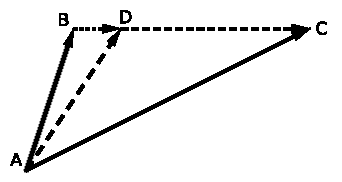
\includegraphics[width=4.0cm]{img/prova-1-pro-fig1}

\item (1,5 pontos) Sabendo que os vetores $\vec{u} + \vec{v}$ e $\vec{u} - \vec{v}$ tem a mesma norma, qual é o ângulo entre $\vec{u}$ e $\vec{v}$? (dica: interprete geometricamente)
\item (1,5 pontos) O ângulo entre cada um dos vetores $\vec{i}$, $\vec{j}$ e $\vec{k}$ da base canônica e um certo vetor unitário $\vec{v}$ é sempre o mesmo. Quais podem ser as coordenadas de $\vec{v}$?
\item (2,0 pontos) Seja $A=(1,-2,1)$, $B$ e $C$ vértices de um triângulo retângulo com ângulo reto em $A$. Determine $B$ e $C$, sabendo que a hipotenusa mede $3\sqrt{2}$, que $\norm{\vect{AB}} = \norm{\vect{AC}}$ e que os catetos $\vect{AB}$ e $\vect{AC}$ têm mesma direção e sentido que $\vec{i}$ e $\vec{k}$, respectivamente.
\end{enumerate}


\section*{Lembrete}
Se o ângulo entre os vetores $\vec{u} = (x_1, y_1, z_1)$ e $\vec{v} = (x_2, y_2, z_2)$ é $\theta$, e $\vec{v}$ forma ângulos $\alpha$, $\beta$ e $\gamma$ com os vetores $\vec{i}$, $\vec{j}$ e $\vec{k}$, respectivamente, então:
\begin{itemize}
\item $\vec{u} \cdot \vec{v} = \norm{\vec{u}} \cdot \norm{\vec{v}} \cdot \cos(\theta) = x_1x_2 + y_1y_2 + z_1z_2$
\item $\norm{\vec{u}} = \sqrt{\vec{u} \cdot \vec{u}} = \sqrt{x_1^2 + y_1^2 + z_1^2}$
\item $\cos(\alpha) = \frac{x_2}{\norm{\vec{v}}}$, $\cos(\beta) = \frac{y_2}{\norm{\vec{v}}}$ e $\cos(\gamma) = \frac{z_2}{\norm{\vec{v}}}$
\item A projeção de $\vec{u}$ sobre $\vec{v}$ é $\text{Proj}_{\vec{v}}\vec{u} = \left( \frac{\vec{u} \cdot \vec{v}}{ \norm{ \vec{v} }^2} \right) \vec{v} $
\end{itemize}



\newpage
\restoregeometry
\section*{Respostas e observações}

\begin{enumerate}
\item \textit{Sejam $A = (-1, -2\sqrt{2}, 1)$, $B = (2, -2\sqrt{2}, 1)$ e $C = (2, \sqrt{2}, 4)$.}
\begin{enumerate}
\item \textit{O triângulo com vértices $A$, $B$ e $C$ é retângulo?}

Podemos obter os seguintes vetores a partir dos pontos dados:
\begin{itemize}
\item $\vect{AB} = B - A
                 = (2, -2\sqrt{2}, 1) - (-1, -2\sqrt{2}, 1)
                 = (3, 0, 0)$
\item $\vect{AC} = C - A
                 = (2, \sqrt{2}, 4) - (-1, -2\sqrt{2}, 1)
                 = (3, 3\sqrt{2}, 3)$
\item $\vect{BC} = C - B
                 = (2, \sqrt{2}, 4) - (2, -2\sqrt{2}, 1)
                 = (0, 3\sqrt{2}, 3)$
\end{itemize}
Cada um deles corresponde a um dos lados do triângulo. Para que ele seja retângulo, dois destes vetores devem ser ortogonais, isto é, o seu produto escalar tem que ser nulo. Estes são os produtos para cada par de vetores:
\begin{itemize}
\item $\vect{AB} \cdot \vect{AC}
     = (3, 0, 0) \cdot (3, 3\sqrt{2}, 3)
     = 3\cdot 3 + 0 \cdot 3\sqrt{2} + 0 \cdot 3
     = 9$
\item $\vect{AC} \cdot \vect{BC}
     = (3, 3\sqrt{2}, 3) \cdot (0, 3\sqrt{2}, 3)
     = 3\cdot 0 + 3\sqrt{2} \cdot 3\sqrt{2} + 3 \cdot 3
     = 27$
\item $\vect{BC} \cdot \vect{AB}
     = (0, 3\sqrt{2}, 3) \cdot (3, 0, 0)
     = 0\cdot 3 + 3\sqrt{2} \cdot 0 + 3 \cdot 0
     = 0$
\end{itemize}
Como $\vect{BC} \cdot \vect{AB} = 0$, estes vetores são ortogonais e o triângulo tem um ângulo reto no vértice $B$.

\textbf{Nota:} Se começar calculando este produto escalar, já poderá concluir que é um triângulo retângulo sem fazer os outros dois produtos.
\item \textit{Qual é a medida do maior lado do triângulo?}

Em um triângulo retângulo, o maior lado é a hipotenusa (o lado oposto ao ângulo reto). No caso, sua medida será o módulo do vetor $\vect{AC}$:
\begin{itemize}
\item  $\norm{\vect{AC}} = \norm{(3, 3\sqrt{2}, 3)} = \sqrt{3^2 + (3\sqrt{2})^2 + 3^2} = \sqrt{36} = 6$
\end{itemize}
\textbf{Nota:} O fato deste ser o maior lado também pode ser comprovado calculando as medidas dos outros lados, e comparando-as:
\begin{itemize}
\item $\norm{\vect{AB}} = \norm{(3, 0, 0)} = \sqrt{3^2 + 0^2 + 0^2} = \sqrt{9} = 3 < 6$
\item $\norm{\vect{BC}} = \norm{(0, 3\sqrt{2}, 3)} = \sqrt{0^2 + (3\sqrt{2})^2 + 3^2} = \sqrt{27} = 3 \sqrt{3} < 6$
\end{itemize}
\item \textit{Quanto mede o menor dos seus ângulos?}

Já foi visto que $\vect{AB}$ e $\vect{BC}$ formam um ângulo de $90\degree$. Já o ângulo $\theta$ entre $\vect{AB}$ e $\vect{AC}$ pode ser obtido da fórmula que relaciona o produto escalar ao ângulo entre os vetores, assim:
\[
\cos(\theta) = \frac{\vect{AB} \cdot \vect{AC}}
                   {\norm{\vect{AB}} \cdot \norm{\vect{AC}}}
            = \frac{9}{3 \cdot 6}
            = \frac{1}{2}.
\]
Logo, $\theta = \arccos\left( \frac{1}{2} \right) = 60 \degree.$ O ângulo que falta, digamos $\theta_2$, pode ser obtido lembrando que a soma dos ângulos internos de um triângulo é igual a $180\degree$, o que significa que $\theta_2 = 180\degree - 90\degree - 60\degree = 30\degree$, de modo que $\theta_2$ é então o menor dos três ângulos.

\textbf{Nota:} Outra alternativa é utilizar novamente a fórmula do produto escalar:
\[
\cos(\theta_2) = \frac{\vect{AC} \cdot \vect{BC}}
                      {\norm{\vect{AC}} \cdot \norm{\vect{BC}}}
            = \frac{27}{6 \cdot 3 \sqrt{3}}
            = \frac{3}{2\sqrt{3}}
            = \frac{\sqrt{3}}{2}.
\]
Logo, $\theta_2 = \arccos\left( \frac{\sqrt{3}}{2} \right) = 30 \degree.$
\item \textit{Quais as coordenadas do vetor $\text{Proj}_{\vect{AC}}\vect{AB}$?}

Pela fórmula da projeção,
\[
\text{Proj}_{\vect{AC}}\vect{AB}
= \left( \frac{\vect{AB} \cdot \vect{AC}}{ \norm{ \vect{AC} }^2} \right) \vect{AC}
= \left( \frac{9}{ 6^2} \right) \vect{AC}
= \frac{1}{4}\vect{AC}
= \frac{1}{4}\left(3, 3\sqrt{2}, 3\right)
= \left(\frac{3}{4}, \frac{3\sqrt{2}}{4}, \frac{3}{4} \right).
\]

\item \textit{Qual é o módulo de $\text{Proj}_{\vect{AC}}\vect{AB}$?}
\[
 \norm{\text{Proj}_{\vect{AC}}\vect{AB}}
= \norm{\frac{1}{4}\vect{AC}}
= \frac{1}{4} \cdot \norm{\vect{AC}}
= \frac{1}{4} \cdot 6
= \frac{3}{2}.
\]
\end{enumerate}
\item \textit{Sejam $B$ e $C$ dois pontos do espaço. Considere o ponto $D$ do segmento de reta $BC$, tal que $\vect{DC} = 5 \vect{BD}$. Se $A$ é um ponto que não pertencente à reta $BC$, escreva o vetor $\vect{AD}$ em termos dos vetores $\vect{AB}$ e $\vect{AC}$ (dica: use somas de vetores apropriados).}

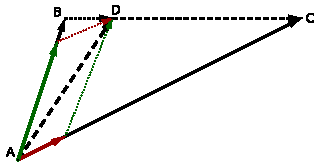
\includegraphics[width=5.0cm]{img/prova-1-pro-fig1b}

Primeiramente, escrevemos $\vect{AD} = \vect{AB} + \vect{BD}$. Como $\vect{DC} = 5 \vect{BD}$, temos $\vect{BD} = \frac{1}{5} \vect{DC}$, que podemos substituir na expressão de $\vect{AD}$ para obter
\[
\vect{AD} = \vect{AB} + \frac{1}{5} \vect{DC}.
\]
Mas este vetor $\vect{DC} = -\vect{AD} + \vect{AC}$, então
\[
\vect{AD} = \vect{AB} + \frac{1}{5} (-\vect{AD} + \vect{AC})
          = \vect{AB} - \frac{1}{5} \vect{AD} + \frac{1}{5} \vect{AC},
\]
e podemos usar a equação anterior para isolar $\vect{AD}$ em função dos outros vetores:
\[
\vect{AD} + \frac{1}{5} \vect{AD} = \vect{AB} + \frac{1}{5} \vect{AC}
\]
\[
\frac{6}{5} \vect{AD} = \vect{AB} + \frac{1}{5} \vect{AC}
\]
\[
\vect{AD} = \frac{5}{6} \vect{AB} + \frac{1}{6} \vect{AC}.
\]

\item \textit{Sabendo que os vetores $\vec{u} + \vec{v}$ e $\vec{u} - \vec{v}$ tem a mesma norma, qual é o ângulo entre $\vec{u}$ e $\vec{v}$? (dica: interprete geometricamente)}

Conforme o enunciado, a norma
\begin{align*}
\norm{\vec{u} + \vec{v}}
& = \sqrt{(\vec{u} + \vec{v}) \cdot (\vec{u} + \vec{v})} \\
& = \sqrt{
    \vec{u} \cdot \vec{u}
  + \vec{u} \cdot \vec{v}
  + \vec{v} \cdot \vec{u}
  + \vec{v} \cdot \vec{v}
} \\
& = \sqrt{
    \vec{u} \cdot \vec{u}
  + 2 (\vec{u} \cdot \vec{v})
  + \vec{v} \cdot \vec{v}
}
\end{align*}
é igual à norma
\[
\norm{\vec{u} - \vec{v}}
= \sqrt{(\vec{u} - \vec{v}) \cdot (\vec{u} - \vec{v})}
= \sqrt{
    \vec{u} \cdot \vec{u}
  - 2 (\vec{u} \cdot \vec{v})
  + \vec{v} \cdot \vec{v}
}.
\]
Podemos eliminar as raízes elevando as duas expressões ao quadrado, obtendo então a igualdade
\[
  \vec{u} \cdot \vec{u}
+ 2 (\vec{u} \cdot \vec{v})
+ \vec{v} \cdot \vec{v}
=
  \vec{u} \cdot \vec{u}
- 2(\vec{u} \cdot \vec{v})
+ \vec{v} \cdot \vec{v}.
\]

Como o objetivo é saber o ângulo entre $\vec{u}$ e $\vec{v}$, e tal ângulo está relacionado ao produto escalar $\vec{u} \cdot \vec{v}$, basta isolar este produto na equação anterior. Para isso, cancelamos os termos $\vec{u} \cdot \vec{u}$ e $\vec{v} \cdot \vec{v}$ em ambos os membros, para obter
\[2 \vec{u} \cdot \vec{v} = - 2 \vec{u} \cdot \vec{v},\]
isto é,
$4 \vec{u} \cdot \vec{v} = 0$. Logo $\vec{u} \cdot \vec{v} = 0$, o que significa que os vetores são ortogonais, ou seja, formam um ângulo de $90\degree$.

\textbf{Nota:} Geometricamente, os únicos paralelogramos determinados por vetores $\vec{u}$ e $\vec{v}$ em que as diagonais $\vec{u} + \vec{v}$ e $\vec{u} - \vec{v}$ têm o mesmo tamanho são os retângulos, isto é, quando o ângulo entre $\vec{u}$ e $\vec{v}$ é de $90\degree$.

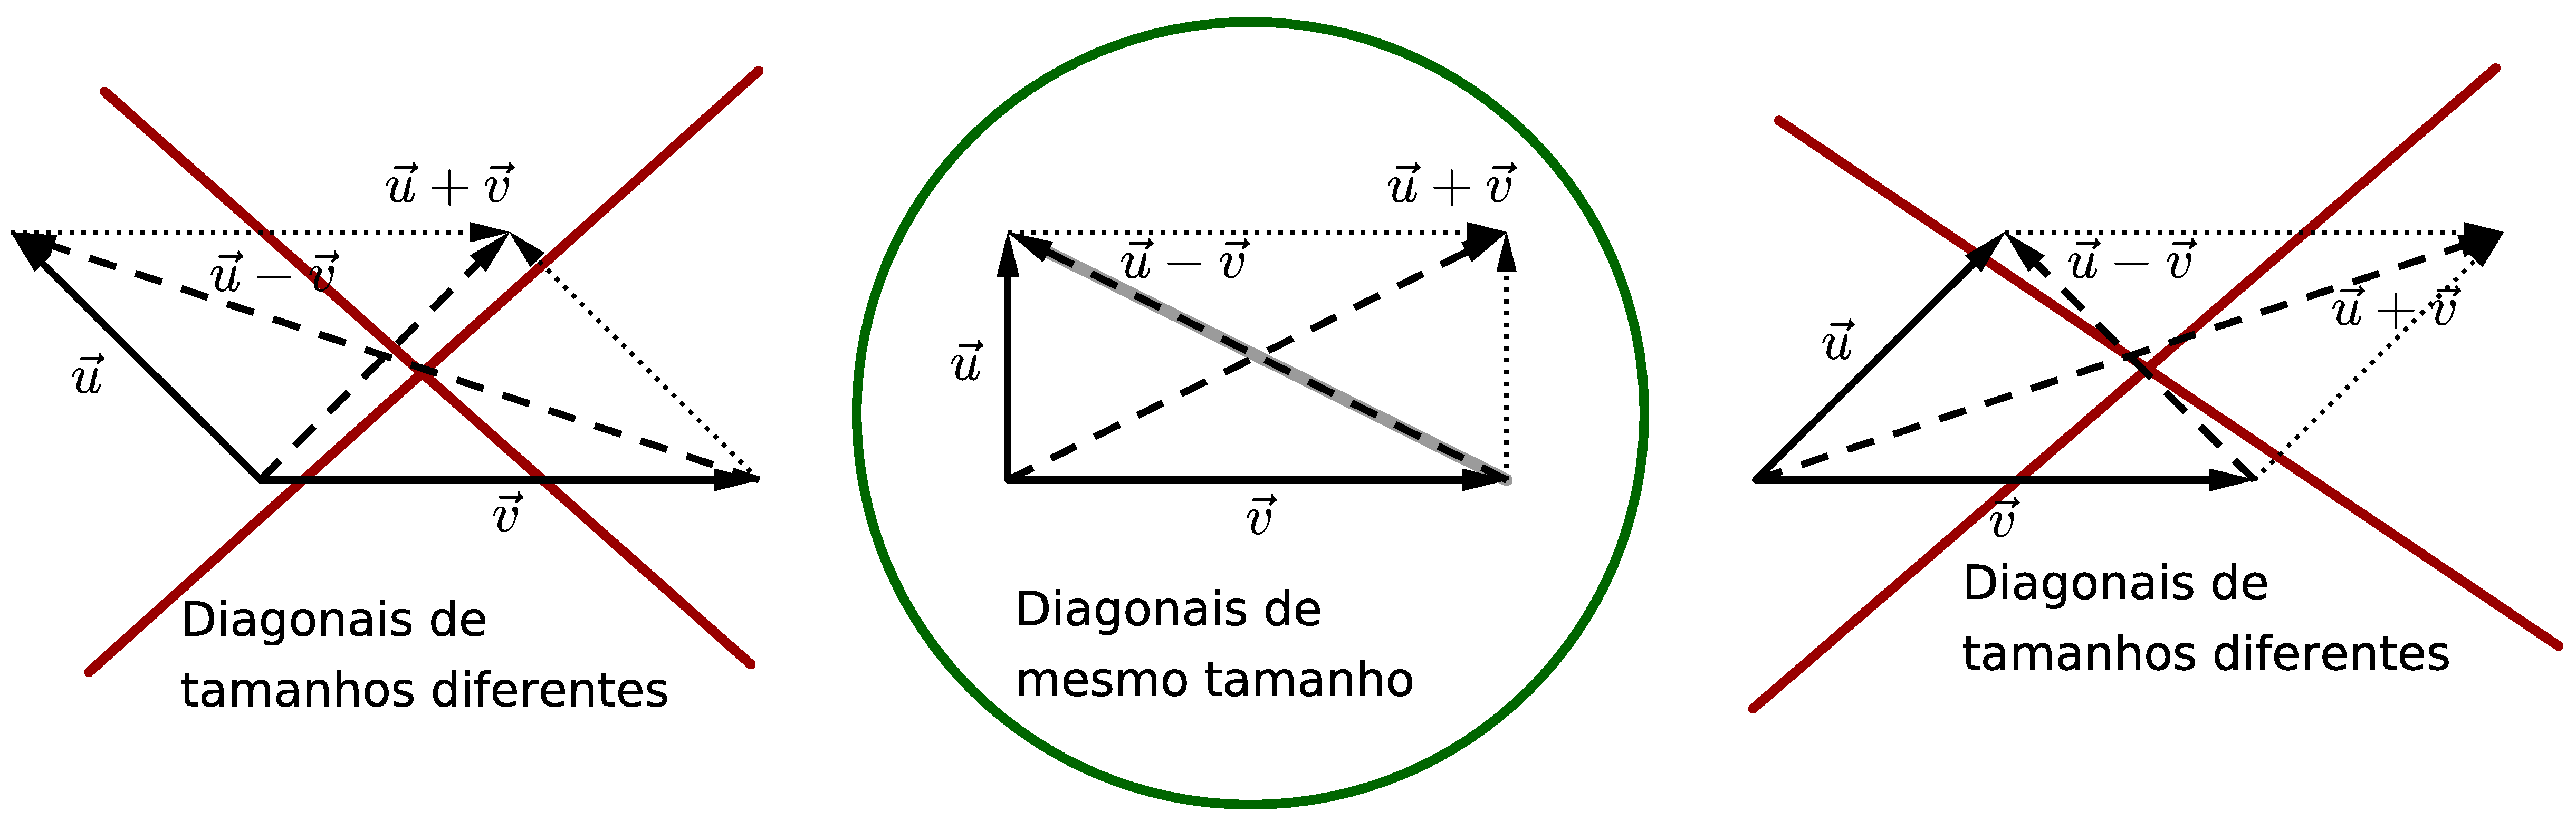
\includegraphics[width=12.0cm]{img/prova-1-pro-fig2}

\item \textit{O ângulo entre cada um dos vetores $\vec{i}$, $\vec{j}$ e $\vec{k}$ da base canônica e um certo vetor unitário $\vec{v}$ é sempre o mesmo. Quais podem ser as coordenadas de $\vec{v}$?}

Os ângulos $\alpha, \beta$ e $\gamma$ que $\vec{v}$ forma com os vetores da base canônica são iguais, então os seus cossenos (os cossenos diretores de $\vec{v}$) também coincidem. Assim,
\[
\cos(\alpha) = \cos(\beta) = \cos(\gamma)
\Rightarrow
  \frac{x}{\norm{\vec{v}}}
= \frac{y}{\norm{\vec{v}}}
= \frac{z}{\norm{\vec{v}}}
\Rightarrow
  x = y = z.
\]
Como o vetor $\vec{v} = (x,y,z)$ é unitário, temos
\[
1 = \norm{ \vec{v} }
  = \sqrt{ x^2 + y^2 + z^2}
  = \sqrt{ x^2 + x^2 + x^2}
  = \sqrt{3 x^2},
\]
ou seja, $3 x^2 = 1$. Logo, $x = \pm \sqrt{\frac{1}{3}} = \pm \frac{1}{\sqrt{3}} = \pm \frac{\sqrt{3}}{3}$ e existem duas possibilidades para $\vec{v}$, que são $\vec{v} = \pm(\frac{\sqrt{3}}{3},\frac{\sqrt{3}}{3},\frac{\sqrt{3}}{3})$.
\item \textit{Seja $A=(1,-2,1)$, $B$ e $C$ vértices de um triângulo retângulo com ângulo reto em $A$. Determine $B$ e $C$, sabendo que a hipotenusa mede $3\sqrt{2}$, que $\norm{\vect{AB}} = \norm{\vect{AC}}$ e que os catetos $\vect{AB}$ e $\vect{AC}$ têm mesma direção e sentido que $\vec{i}$ e $\vec{k}$, respectivamente.}

Podemos visualizar os dados fornecidos com o auxílio do seguinte triângulo retângulo, com um ângulo reto em $A$ e catetos de mesmo comprimento:

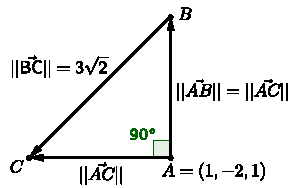
\includegraphics[width=6.0cm]{img/prova-1-pro-fig3}

Por Pitágoras, temos
\[
\norm{\vect{BC}}^2
= \norm{\vect{AB}}^2 + \norm{\vect{AC}}^2
= \norm{\vect{AC}}^2 + \norm{\vect{AC}}^2
= 2 \norm{\vect{AC}}^2.
\]
Então $2 \norm{\vect{AC}}^2 = (3\sqrt{2})^2 = 18$ e resulta que $\norm{\vect{AC}}^2 = 9$, isto é, $\norm{\vect{AC}} = 3 = \norm{\vect{AB}}$.


Como $\vect{AB}$ tem a mesma direção e sentido que o vetor $\vec{i}$, e módulo igual a 3, então $\vect{AB} = 3\vec{i}$. Analogamente, $\vect{AC}$ tem a mesma direção e sentido que o vetor $\vec{k}$ e módulo igual a 3, portanto $\vect{AC} = 3\vec{j} = (0,0,3)$.

Assim, se $B=(x_1,y_1,z_1)$ devemos ter
\[
(3,0,0) = \vect{AB}
        = B-A
        = (x_1, y_1, z_1) - (1,-2,1)
        = (x_1 - 1,y_1 + 2,z_1 - 1),
\]
e portanto $x_1 - 1 = 3$, $y_1 + 2 = 0$, e $z_1 - 1 = 0$, ou seja, $B = (4,-2,1)$. Do mesmo modo, se $C=(x_2,y_2,z_2)$ então
\[
(0,0,3) = \vect{AC}
        = C-A
        = (x_2, y_2, z_2) - (1,-2,1)
        = (x_2 - 1, y_2 + 2, z_2 - 1),
\]
o que significa que $x_2 - 1 = 0$, $y_2 + 2 = 0$, e $z_2 - 1 = 3$, isto é, $C = (1,-2,4)$.
\end{enumerate}
\end{document}
